\section{Introduction}
Mandatory. Questions like: What is the topic of this work, what's the broader context (topic of the proseminar), why is it relevant?

\begin{itemize}
    \item History of ensemble learning + papers of people "inventing" it
    \item Goal of the report
    \item learning more about bagging + boosting
    \item get to know most popular types of both methods
    \item learn how to practically use them
    \item when to use which technique
    \item 
\end{itemize}
% ---------------------------------------------------------------------------- %
\section{Ensemble Learning}
\begin{itemize}
    \item Whats ensemble learning?
    \item wisdom of crowds
\end{itemize}

\subsection{Bagging}
\begin{itemize}
    \item Whats the idea behind it?
    \item How to train bagging? (+ graphic)
    \item How does the prediction work? (+ graphic)
    \item when to use it
    \item advantages and challenges
\end{itemize}

\subsection{Random Forest}
\begin{itemize}
    \item difference to bagging
\end{itemize}

\subsection{Out-of-bag}
\begin{itemize}
    \item explain
\end{itemize}

\subsection{Boosting}
\begin{itemize}
    \item Whats the idea behind it?
    \item How to train boosting? (+ graphic)
    \item How does the prediction work? (+ graphic)
    \item when to use it
    \item advantages and challenges of using it
\end{itemize}

\subsection{Gradient Boosting}
\begin{itemize}
    \item difference to boosting
\end{itemize}

\subsection{Extreme Gradient Boosting}
\begin{itemize}
    \item difference to gradient boosting
\end{itemize}


% ---------------------------------------------------------------------------- %
\section{Examples}
\subsection{Example 1}
\subsection{Example 2}

% ---------------------------------------------------------------------------- %
\section{Summary and conclusion}
Mandatory. Short summary of the most important aspects of the report.
If possible: What are open challenges?

\begin{itemize}
    \item Bagging vs. Boosting - whats the difference?
\end{itemize}

%\newpage
%\section{\LaTeX Examples}
%As a help to get started with this template. To be deleted for submission.
%\subsection{Citation examples}
%\citet{campbell:2017} define the stages of information processing in a nervous system as: "sensory input, integration, and motor output". \\
%The stages of information processing in a nervous system are defined as: "sensory input, integration, and motor output" \citep{campbell:2017}. 
%
%\subsection{Table example}
%\begin{table}[htbp]
    \centering
    \begin{tabular}{lrl}
    \toprule
    labels   & numbers & annotation \\
    \midrule
    abra     &  1.23   & \textbf{this is important}\\
    cadabra  &  2.34   & this isn't\\
    \bottomrule
    \end{tabular}
    \caption{Some random numbers}
    \label{tab:random}
\end{table}
%
%\subsection{Figure examples}
%This is a png file, it gets blurry when you zoom in:
%\begin{figure}[htbp]
%    \centering
%    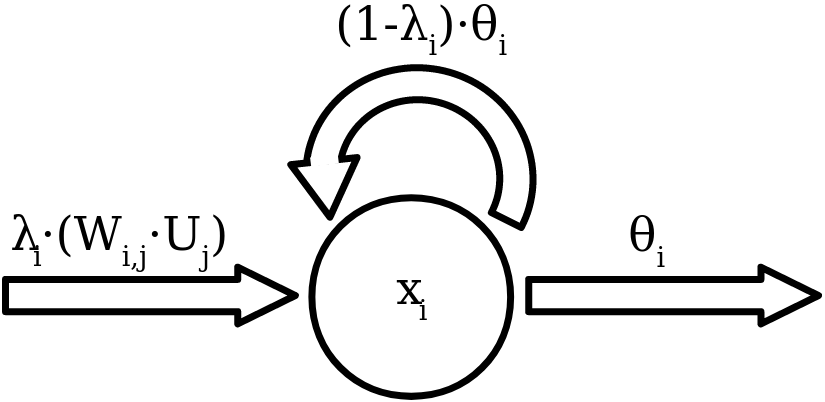
\includegraphics[width=.7\textwidth]{figures/leaky_integration.png}
%    \caption{Symbolic representation of a leaky integrating neuron.}
%    \label{fig:leaky_integration}
%\end{figure}
%
%This is an eps file, it is always sharp:\\
%Notice how the formatting option "[htbp]" allows for the figure to be moved around to page \pageref{fig:activation_function}. Hence, it is best to rather write: The eps file in figure \ref{fig:activation_function} always stays sharp.
%\begin{figure}[htbp]
%    \centering
%    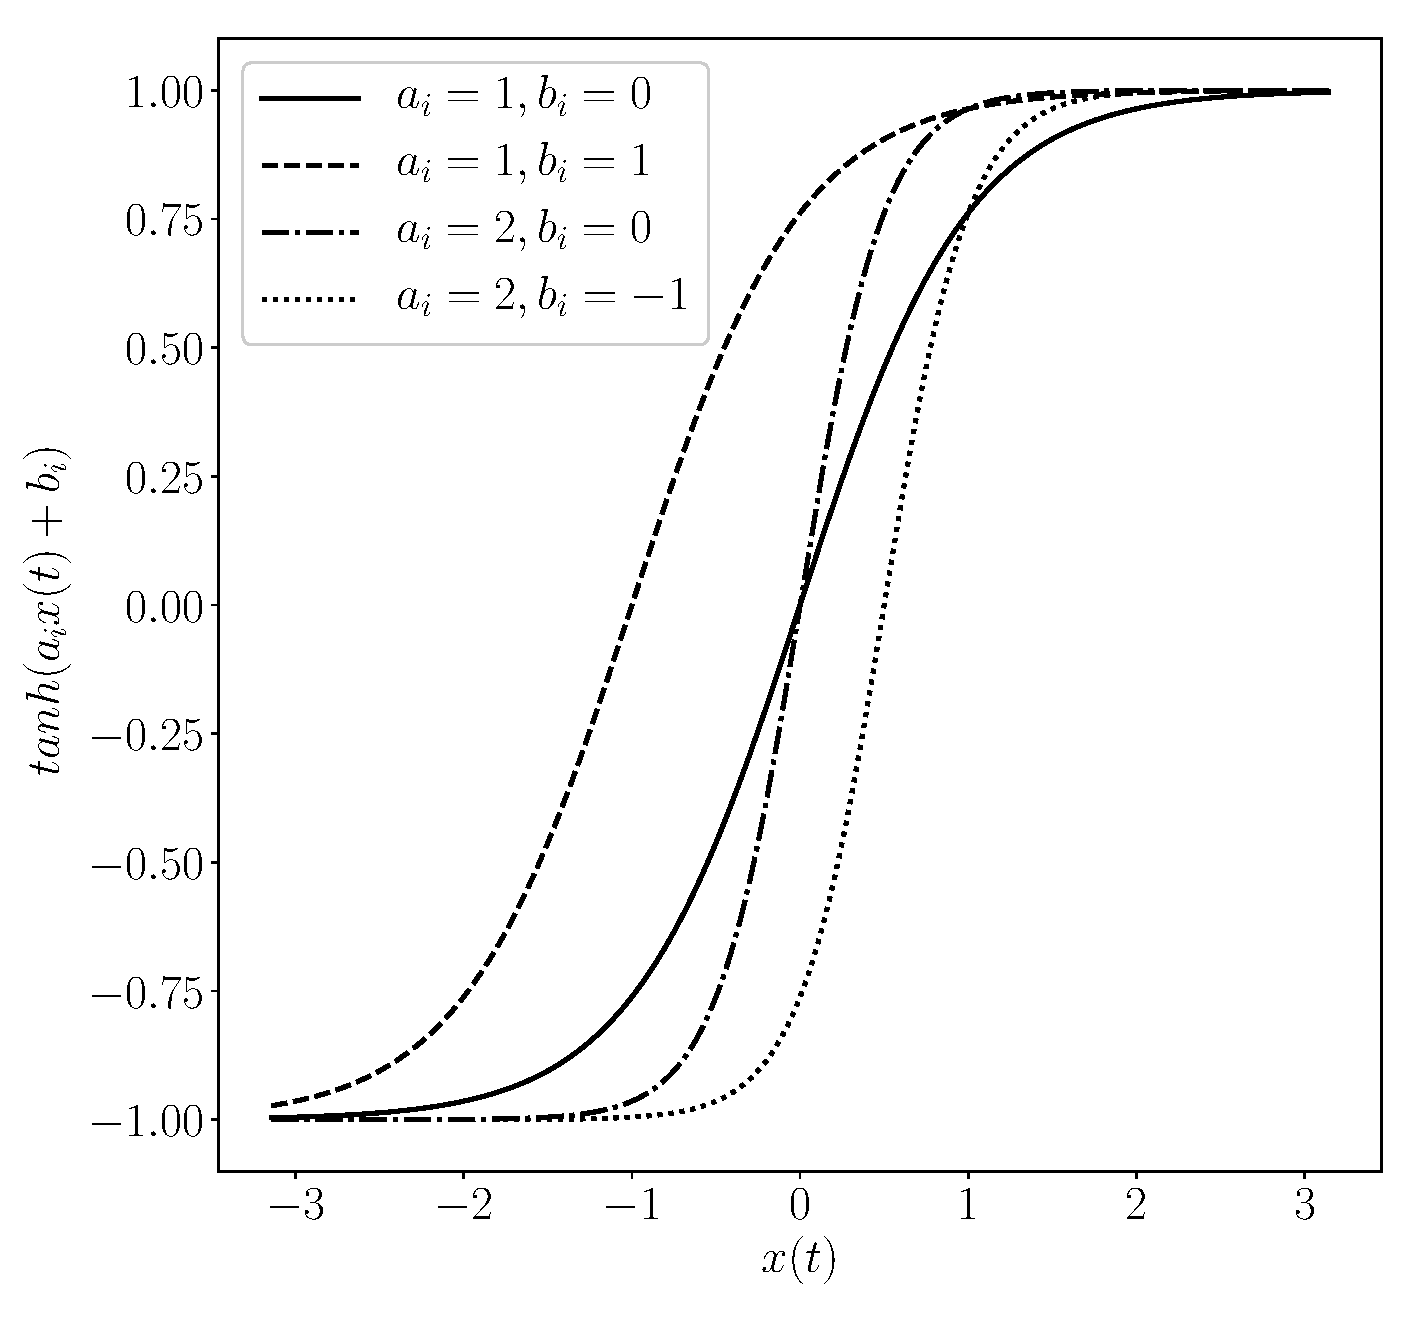
\includegraphics[width=.7\textwidth]{figures/activation_functions}
%    \caption{Shapes of a parametrized tanh activation function.}
%    \label{fig:activation_function}
%\end{figure}
%
%\subsection{Math example}
%The state update of the leaky integrating neuron in figure \ref{fig:leaky_integration} can be formulated as:
%\begin{align}
%    x_i(t+1) &= \lambda_i \cdot \left(W_{i,j} \cdot U_j(t)\right) + (1-\lambda_i) \cdot \theta_i(t)
%    \label{eq:leaky_integration}
%\end{align}
%
%\subsection{Code block example}
%From equation \ref{eq:leaky_integration} the neuron model is implemented using numpy \citep{harris:2020}:
%
%\lstinputlisting[label=py:leaky, language=Python, caption=Python implementation of a single leaky-integrating neuron.]{code/leaky.py}
%
%\subsection{Footnote example}
%The implementation is available on github\footnote{https://github.com/schniewmatz/recurrence}.